\documentclass[12pt]{article}

\usepackage{amsmath}
\usepackage{amssymb}
\usepackage{amsthm}
\usepackage[pdftex]{graphicx}
\usepackage{setspace}
\usepackage{caption}
\usepackage{subcaption}
\usepackage{float}
\usepackage[margin=1in]{geometry}
\usepackage{listings}
\usepackage{textcomp}
\usepackage{multicol}
\usepackage[toc,page]{appendix}
\usepackage{listings}
\usepackage{fancyvrb}
\usepackage{hyperref}
\usepackage{lstbayes}

\usepackage[usenames,dvipsnames]{color}
\definecolor{DGrey}{gray}{0.25}
\definecolor{MGrey}{gray}{0.50}
\definecolor{LGrey}{gray}{0.75}

%\usepackage{algorithm}
%\usepackage{algpseudocode}
\usepackage[ruled,vlined,linesnumbered]{algorithm2e}
\newcommand\mycommfont[1]{\footnotesize\ttfamily\textcolor{Gray}{#1}}
\SetCommentSty{mycommfont}
%\floatname{algorithm}{Procedure}
%\renewcommand{\algorithmicrequire}{\textbf{Input:}}
%\renewcommand{\algorithmicensure}{\textbf{Output:}}
%\makeatletter
%\def\therule{%
%  \makebox[\algorithmicindent][l]{%
%    \hspace*{.5em}\vrule height .75\baselineskip depth .25\baselineskip}}%

\usepackage{inconsolata}

\usepackage[parfill]{parskip}
\setlength{\parindent}{0pt}
\setlength{\parskip}{\baselineskip}

\newcommand{\et}{e^{i\theta}}
\newcommand{\oo}{\mathcal{O}}
\newcommand{\skipline}{\bigskip\bigskip\bigskip}

\lstdefinestyle{Rsty} { 
    language=R,                         % the language of the code
    basicstyle=\footnotesize\ttfamily,  % the size of the fonts that are used for the code
    numbers=left,                       % where to put the line-numbers
    numberstyle=\footnotesize\color{LGrey},      % the style that is used for the line-numbers
    stepnumber=1,                       % the step between two line-numbers. If it is 1, each line
                                        % will be numbered
    numbersep=5pt,                      % how far the line-numbers are from the code
    backgroundcolor=\color{white},      % choose the background color. You must add \usepackage{color}
    showspaces=false,                   % show spaces adding particular underscores
    showstringspaces=false,             % underline spaces within strings
    showtabs=false,                     % show tabs within strings adding particular underscores
    frame=single,                       % adds a frame around the code
    rulecolor=\color{black},            % if not set, the frame-color may be changed on line-breaks within not-black text (e.g. commens (green here))
    tabsize=2,                          % sets default tabsize to 2 spaces
    captionpos=b,                       % sets the caption-position to bottom
    breaklines=true,                    % sets automatic line breaking
    breakatwhitespace=false,            % sets if automatic breaks should only happen at whitespace
    keywordstyle=\color{DGrey},     % keyword style
    commentstyle=\color{LGrey},   % comment style
    stringstyle=\color{MGrey},    % string literal style
    literate={<-}{{$\gets$}}1,           % prettier assignment arrows
    xleftmargin=4.0ex,
    deletekeywords={I,density,rect,_,palette,data,scale,panel,R,frame,labels,options}
}

\lstnewenvironment{R}
{\lstset{style=Rsty}}
{}


\lstdefinestyle{Cppsty} { 
    language=C++,                         % the language of the code
    basicstyle=\footnotesize\ttfamily,  % the size of the fonts that are used for the code
    numbers=left,                       % where to put the line-numbers
    numberstyle=\footnotesize\color{LGrey},      % the style that is used for the line-numbers
    stepnumber=1,                       % the step between two line-numbers. If it is 1, each line
                                        % will be numbered
    numbersep=5pt,                      % how far the line-numbers are from the code
    backgroundcolor=\color{white},      % choose the background color. You must add \usepackage{color}
    showspaces=false,                   % show spaces adding particular underscores
    showstringspaces=false,             % underline spaces within strings
    showtabs=false,                     % show tabs within strings adding particular underscores
    frame=single,                       % adds a frame around the code
    rulecolor=\color{black},            % if not set, the frame-color may be changed on line-breaks within not-black text (e.g. commens (green here))
    tabsize=4,                          % sets default tabsize to 2 spaces
    captionpos=b,                       % sets the caption-position to bottom
    breaklines=true,                    % sets automatic line breaking
    breakatwhitespace=false,            % sets if automatic breaks should only happen at whitespace
    keywordstyle=\color{DGrey},     % keyword style
    commentstyle=\color{LGrey},   % comment style
    stringstyle=\color{MGrey},    % string literal style
    %literate={<-}{{$\gets$}}1,           % prettier assignment arrows
    xleftmargin=4.0ex,
    deletekeywords={T}
}

\lstnewenvironment{Stan}
{\lstset{style=Stansty}}
{}

\renewcommand{\arraystretch}{2}

\begin{document}

\noindent
{\LARGE {\bf Particle Filters} }
\\\\
Dexter Barrows\\
\today

\section{Intro}

	Particle filters are similar to MCMC-based methods in that they attempt to draw samples from an approximation of the posterior distribution of model parameters $\theta$ given observed data $D$. Instead of constructing a Markov chain and approximating its stationary distribution, a cohort of ``particles'' are used to move through the data in an on-line (sequential) fashion with the cohort being culled of poorly-performing particles at each iteration via importance sampling. If the culled particles are not replenished, this will be a Sequential Importance Sampling (SIS) particle filter. If the culled particles are replenished from surviving particles, in a sense setting up a process not dissimilar from Darwinian selection, then this will be a Sequential Importance Resampling (SIR) particle filter.

\section{Formulation}

	Particle filters, also called Sequential Monte-Carlo (SMC) or bootstrap filters, feature similar core functionality as the venerable Kalman Filter. As the algorithm moves through the data (sequence of observations), a prediction-update cycle is used to simulate the evolution of the model $M$ with different particular parameter selections, track how closely these predictions approximate the new observed value, and update the current cohort appropriately.

	Two separate functions are used to simulate the evolution and observation processes. The ``true'' state evolution is specified by

	\begin{equation}
		X_{t+1} \sim f_1 (X_t, \theta),
	\end{equation}

	And the observation process by

	\begin{equation}
		Y_t \sim f_2 (X_t, \theta).
	\end{equation}

	Note that components of $\theta$ can contribute to both functions, but a typical formulation is to have some components contribute to $f_1 (\cdot, \theta)$ and others to $f_2 (\cdot,\theta)$.

	The prediction part of the cycle utilises $f_1 (\cdot, \theta)$ to update each particle's current state estimate to the next time step, while $f_2 (\cdot, \theta)$ is used to evaluate a weighting $w$ for each particle which will be used to determine how closely that particle is estimating the true underlying state of the system. Note that $f_2 (\cdot, \theta)$ could be thought of as a probability of observing a piece of data $y_t$ given the particle's current state estimate and parameter set, $P(y_t | X_t, \theta)$. Then, the new cohort of particles is drawn from the old cohort proportional to the weights. This process is repeated until the set of observations $D$ is exhausted.


\section{Algorithm}

    Now we will formalize the particle filter.

    We will denote each particle $p^{(j)}$ as the $j^{th}$ particle consisting of a state estimate at time $t$, $X_t^{(j)}$, a parameter set $\theta^{(j)}$, and a weight $w^{(j)}$. Note that the state estimates will evolve with the system as the cohort traverses the data.

    The algorithm for a Sequential Importance Resampling particle is shown in Algorithm \ref{pfsir}.\\
    
    \begin{algorithm}[H]

        \BlankLine

        \SetKwInOut{Input}{Input}
        \SetKwInOut{Output}{Output}
        \DontPrintSemicolon

        \tcc{Select a starting point}
        \Input{Observations $D = y_1, y_2, ..., y_T$, initial particle distribution $P_0$ of size $J$}

        \BlankLine

        \tcc{Setup}
        Initialize particle cohort by sampling $(p^{(1)}, p^{(2)}, ..., p^{(J)})$ from $P_0$

        \BlankLine

        \For{$t = 1:T$}{

            \BlankLine

            \tcc{Evolve}
            \For{j = 1:J}{
            	$X_t^{(j)} \gets f_1 (X_{t-1}^{(j)}, \theta^{(j)})$
            }

            \BlankLine

            \tcc{Weight}
            \For{j = 1:J}{
            	$w^{(j)} \gets P(y_t | X_t^{(j)}, \theta^{(j)}) = f_2 (X_t^{(j)}, \theta^{(j)})$
            }

            \BlankLine

            \tcc{Normalize}
            \For{j = 1:J}{
            	$w^{(j)} \gets w^{(j)} / \sum_{1}^{J} w^{(j)}$
            }

            \BlankLine

            \tcc{Resample}
            $p^{(1:J)} \gets \text{sample}(p^{(1:J)}, \text{prob} = w, \text{replace} = true)$
        }

        \BlankLine

        \tcc{Samples from approximated posterior distribution}
        \Output{Cohort of posterior samples $(\theta^{(1)},\theta^{(2)},...,\theta^{(J)})$}

        \BlankLine

        \caption{SIR particle filter}\label{pfsir}

    \end{algorithm}

\section{Particle Collapse}

	Not uncommonly, a situation may arise in which a single particle is assigned a normalized weight very close to 1 and all the other particles are assigned weights very close to 0. When this occurs, the next generation of the cohort will overwhelmingly consist of descendants of the heavily-weighted particle, termed particle collapse or degeneracy.

	Since the basic SIR particle filter does not perturb either the particle system states or system parameter values, the cohort will quickly consist solely of identical particles, effectively halting further exploration of the parameter space as new data is introduced.

	A similar situation occurs when a small number of particles (but not necessarily a single particle) split almost all of the normalized weight between them, then jointly dominate the resampling process for the remainder of the iterations. This again halts the exploration of the parameter space with new data.

	In either case, the hallmark feature used to detect collapse is the same -- at some point the cohort will consist of particles with very similar or identical parameter sets which will consequently result in their assigned weights being extremely close together.

	Mathematically, we are interested in the number of effective particles, $N_{eff}$, which represents the number of particles that are acceptably dissimilar. This is estimated by evaluating

	\begin{equation}
		N_{eff} = \frac{1}{\sum_1^J (w^{(j)})^2}.
	\end{equation}

	This can be used to diagnose not only when collapse has occurred, but can also indicate when it is near.

\section{Iterated Filtering and Data Cloning}

	A particle filter hinges on the idea that as it progresses through the data set $D$, its estimate of the posterior carried in the cohort of particles approaches maximum likelihood. However, this convergence may not be fast enough so that the estimate it produces is of quality before the data runs out. One way around this problem is to ``clone'' the data and make multiple passes through it as if it were a continuation of the original time series. Note that the system state contained in each particle will have to be reset with each pass.

	Rigorous proofs have been developed (references to Ionides et. al. work) that show that by treating the parameters as stochastic processes instead of fixed values, the multiple passes through the data will indeed force convergence of the process mean toward maximum likelihood, and the process variance toward 0.

\section{IF2}

	The successor to Iterated Filtering 1 (reference), Iterated Filtering 2 is simpler, faster, and demonstrated better convergence toward maximum likelihood (reference). The core concept involves a two-pronged approach. First, Data cloning is used to allow more time for the parameter stochastic process means to converge to maximum likelihood, and frequent cooled perturbation of the particle parameters allow better exploration of the parameter space while still allowing convergence to good point estimates.

	It is worth noting that IF2 is not designed to estimate the full posterior distribution, but in practice can be used to do so within reason. Further, IF2 thwarts the problem of particle collapse by keeping at least some perturbation in the system at all times. It is important to note that while true particle collapse will not occur, there is still risk of a pseudo-collapse in which all particles will be extremely close to one another so as to be virtually indistinguishable. However this will only occur with the use of overly-aggressive cooling strategies or by specifying an excessive number of passes through the data.

	An important new quantity is the particle perturbation density denoted $h(\theta|,\sigma)$. Typically this is multi-normal with $\sigma$ being a vector of variances proportional to the expected values of $\theta$. In practice the proportionality can be derived from current means or specified ahead of time. Further, these intensities must decrease over time. This can be done via exponential or geometric cooling, a decreasing step function, a combination of these, or though some other similar scheme.

	The algorithm for IF2 can be seen in Algorithm \ref{if2}.\\

    \begin{algorithm}[H]

        \BlankLine

        \SetKwInOut{Input}{Input}
        \SetKwInOut{Output}{Output}
        \DontPrintSemicolon

        \tcc{Select a starting point}
        \Input{Observations $D = y_1, y_2, ..., y_T$, initial particle distribution $P_0$ of size $J$, decreasing sequence of perturbation intensity vectors $\sigma_1, \sigma_2, ..., \sigma_M$}

        \BlankLine

        \tcc{Setup}
        Initialize particle cohort by sampling $(p^{(1)}, p^{(2)}, ..., p^{(J)})$ from $P_0$

        \BlankLine

        \tcc{Particle seeding distribution}
        $\Theta \gets P_0$

        \BlankLine

        \For{$m = 1:M$}{

        	\BlankLine

        	\tcc{Pass perturbation}
            \For{j = 1:J}{
            	$p^{(j)} \sim h(\Theta^{(j)}, \sigma_m)$
            }

            \BlankLine

	        \For{$t = 1:T$}{

	        	\BlankLine
	        	
		        \For{j = 1:J}{

		        	\BlankLine
		        	\tcc{Iteration perturbation}
	            	$p^{(j)} \sim h(p^{(j)}, \sigma_m)$

	            	\BlankLine
	            	\tcc{Evolve}
	            	$X_t^{(j)} \gets f_1 (X_{t-1}^{(j)}, \theta^{(j)})$

	            	\BlankLine
	            	\tcc{Weight}
	            	$w^{(j)} \gets P(y_t | X_t^{(j)}, \theta^{(j)}) = f_2 (X_t^{(j)}, \theta^{(j)})$

	            }

	            \BlankLine

	            \tcc{Normalize}
	            \For{j = 1:J}{
	            	$w^{(j)} \gets w^{(j)} / \sum_{1}^{J} w^{(j)}$
	            }

	            \BlankLine

	            \tcc{Resample}
	            $p^{(1:J)} \gets \text{sample}(p^{(1:J)}, \text{prob} = w, \text{replace} = true)$

	        }

	        \BlankLine

	        \tcc{Collect particles for next pass}
	        \For{$j = 1:J$}{
	        	$\Theta^{(j)} \gets p^{(j)}$
	        }

	    }

        \BlankLine

        \tcc{Samples from approximated posterior distribution}
        \Output{Cohort of posterior samples $(\theta^{(1)},\theta^{(2)},...,\theta^{(J)})$}

        \BlankLine

        \caption{IF2}\label{if2}

    \end{algorithm}



\section{Fitting an SIR Model to Synthetic Epidemic Data with IF2}

    Here we will examine a test case in which IF2 will be used to fit a Susceptible-Infected-Removed (SIR) epidemic model to mock infectious count data.

    The synthetic data was produced by taking the solution to a basic SIR ODE model, sampling it at regular intervals, and perturbing those values by adding in observation noise. The SIR model used was

    \begin{equation}
        \begin{array}{rl}
            \dfrac{dS}{dt} & = - \beta I S \\
            \dfrac{dI}{dt} & = \beta I S - rI  \\
            \dfrac{dR}{dt} & = rI
        \end{array}
    \end{equation}

    where $S$ is the number of individuals susceptible to infection, $I$ is the number of infectious individuals, $R$ is the number of recovered individuals, $\beta = R_0 r / N$ is the force of infection, $R_0$ is the number of secondary cases per infected individual, $r$ is the recovery rate, and $N$ is the population size.

    The solution to this system was obtained using the \verb|ode()| function from the \verb|deSolve| package. The required derivative array function in the format required by \verb|ode()| was specified as

    \begin{R}    
    SIR <- function(Time, State, Pars) {

        with(as.list(c(State, Pars)), {
            
            B   <- R0*r/N    # calculate Beta
            BSI <- B*S*I     # save product
            rI  <- r*I       # save product
            
            dS = -BSI       # change in Susceptible people
            dI = BSI - rI   # change in Infected people
            dR = rI         # change in Removed (recovered people)
            
            return(list(c(dS, dI, dR)))
            
        })
        
    }
    \end{R}

    The true parameter values were set to $R_0 = 3.0, r = 0.1, N = 500$ by

    \begin{R}
    pars  <- c(R0  = 3.0,  # new infected people per infected person
              r   = 0.1,  # recovery rate
              N   = 500)  # population size
    \end{R}

    The initial conditions were set to 5 infectious individuals, 495 people susceptible to infection, and no one had yet recovered from infection and been removed. These were set using

    \begin{R}
	true_init_cond <- c(S = N - i_infec,
                	   I = i_infec,
                	   R = 0)
    \end{R}

    The \verb|ode()| function is called as

    \begin{R}
    odeout <- ode(y = true_init_cond, times = 0:(T-1), func = SIR, parms = true_pars)
    \end{R}

    where \verb|odeout| is a $T \times 4$ matrix where the rows correspond to solutions at the given times (the first row is the initial condition), and the columns correspond to the solution times and S-I-R counts at those times.

    The observation error was taken to be $\varepsilon_{obs} \sim \mathcal{N}(0,\sigma)$, where individual values were drawn for each synthetic data point.

    These ``true'' values were perturbed to mimic observation error by

    \begin{R}
    set.seed(1001)  # set RNG seed for reproducibility
    sigma <- 10      # observation error standard deviation
    infec_counts_raw <- odeout[,3] + rnorm(101, 0, sigma)
    infec_counts     <- ifelse(infec_counts_raw < 0, 0, infec_counts)
    \end{R}

    where the last two lines simply set negative observations (impossible) to 0.

    Plotting the data using the \verb|ggplot2| package by

    \begin{R}
    plotdata <- data.frame(times=1:T,true=trueTraj,data=infec_counts)

	  g <- ggplot(plotdata, aes(times)) +
	        geom_line(aes(y = true, colour = "True")) +
	        geom_point(aes(y = data, color = "Data")) +
	        labs(x = "Time", y = "Infection count", color = "") +
	        scale_color_brewer(palette="Paired") +
	        theme(panel.background = element_rect(fill = "#F0F0F0"))
    \end{R}

    we obtain Figure \ref{dataplot}.

    \begin{figure}[H]
        \centering
        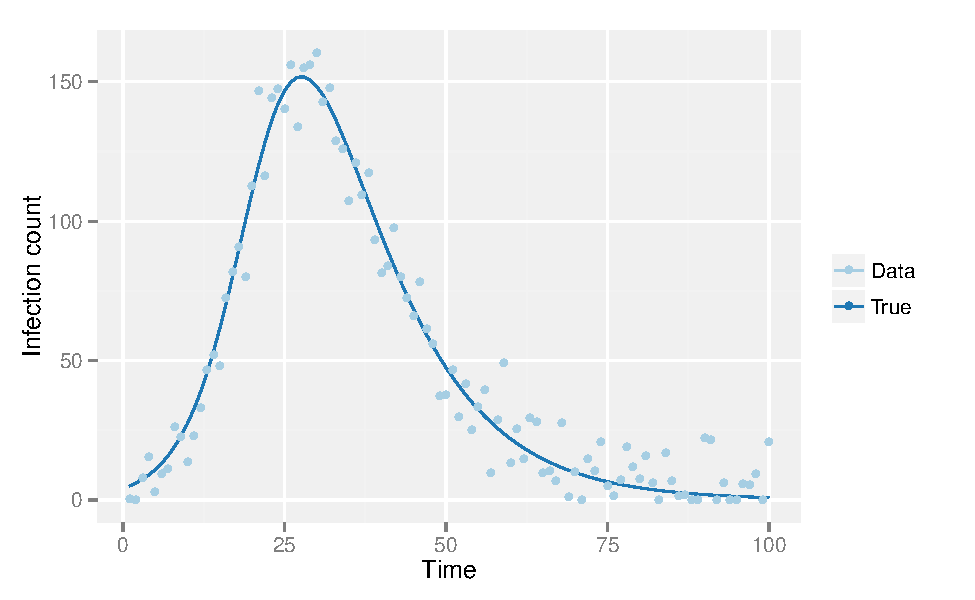
\includegraphics[width=\textwidth]{./images/dataplot.pdf}
        \caption{True SIR ODE solution infected counts, and with added observation noise}
        \label{dataplot}
    \end{figure}

    The IF2 algorithm was implemented in C++ for speed, and integrated into the R workflow using the \verb|Rcpp| package. The C++ code is compiled using

    \begin{R}
    sourceCpp(paste(getwd(),"if2.cpp",sep="/"))
    \end{R}

    Then run and packed into a data frame using

    \begin{R}
    paramdata <- data.frame(if2(infec_counts[1:Tlim], Tlim, N))
	  colnames(paramdata) <- c("R0", "r", "sigma", "Sinit", "Iinit", "Rinit")
    \end{R}

    The final kernel estimates for four of the key parameters are shown in Figure \ref{kernelplot}.

    \begin{figure}[H]
        \centering
        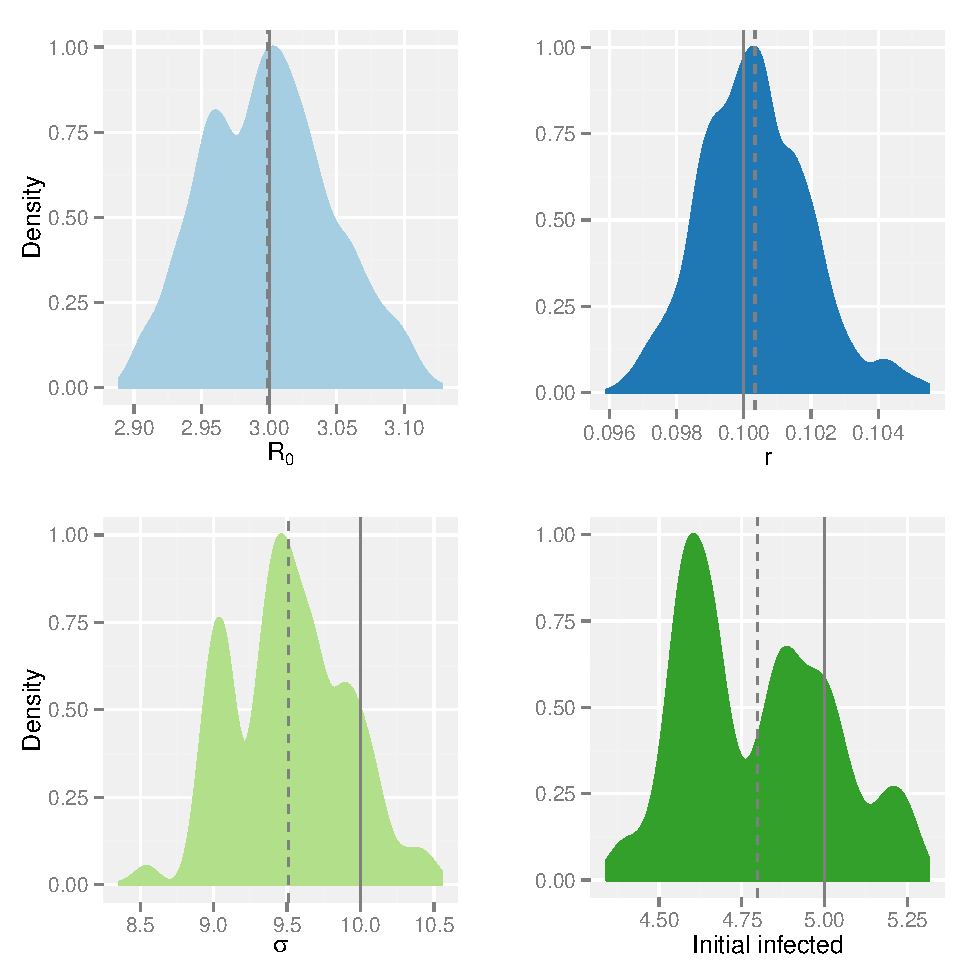
\includegraphics[width=\textwidth]{./images/if2kernels.pdf}
        \caption{Kernel estimates for four essential system parameters. True values are indicated by solid vertical lines, sample means by dashed lines.}
        \label{kernelplot}
    \end{figure}


\newpage
\begin{appendices}

	\section{Full R code}

    This code will run all the indicated analysis and produce all plots.

    \lstinputlisting[style=Rsty]{../../code/if2/d_sir_if2.r}

    \section{Full C++ code}

    Stan model code to be used with the preceding R code.

    \lstinputlisting[style=Cppsty]{../../code/if2/d_if2.cpp}

\end{appendices}







\end{document}